\documentclass[a4paper,12pt]{report}
\usepackage[a4paper, left=2.5cm, right=2.5cm, top=2.5cm, bottom=2.5cm]{geometry}
\usepackage{graphicx}
\usepackage{geometry}
\usepackage{float}
\usepackage{amsmath}
\usepackage{titlesec} 
\usepackage{lipsum}  
\usepackage{hyperref}
\usepackage{nameref}
\usepackage{xcolor}
\usepackage{etoolbox}
\usepackage{blindtext}
\usepackage{tocloft}
\usepackage{textcomp}
\usepackage{url}
\usepackage{caption}
\graphicspath{{fig/}}
\usepackage{chngcntr}
\counterwithout{table}{chapter}






%%%%%%%%%%%%%%%%%%%%%%%%%%%%%%%%%%%%%%%%%%%%This will cause your sections/chapters/subsections to be numbered or not play artound 
\setcounter{secnumdepth}{2}
\setlength{\cftbeforetoctitleskip}{0em}
\setlength{\cftbeforeloftitleskip}{0em}\setlength{\cftbeforelottitleskip}{0em}
%%%%%%%%%%%%%%%%%%%%%%%%%%%%%%%%%%%%%%%%%%%

%%%%%%%%%%%%%%%%%%%%%%%%%%%%%%%%%%%%%%%%%%%
%This simply makes it sotaht there is not a large margin at the top of a new page
%%%%%%%%%%%%%%%%%%%%%%%%%%%%%%%%%%%%%%%%%%%%%%%
\makeatletter
\renewcommand*\@makechapterhead[1]{%
   %\vspace*{50\p@}%
   {\parindent \z@ \raggedright \normalfont
     \ifnum \c@secnumdepth >\m@ne
         \huge\bfseries \@chapapp\space \thechapter
         \par\nobreak
         \vskip 20\p@
     \fi
     \interlinepenalty\@M
     \Huge \bfseries #1\par\nobreak
     \vskip 40\p@
   }}
\renewcommand*\@makeschapterhead[1]{%
   %\vspace*{50\p@}%
   {\parindent \z@ \raggedright
     \normalfont
     \interlinepenalty\@M
     \Huge \bfseries  #1\par\nobreak
     \vskip 40\p@
   }}
\makeatother
%%%%%%%%%%%%%%%%%%%%%%%%%%%%%%%%%%%%%%%%%%%%%%%%%%%%%%%%%%

%%%%%%%%%%%%%%%%%%%%%%%%%%%This makes the list of symbol and abbreviations also have a nice dot fill%%%%%%%%%%%%%%%%%
\makeatletter
\newcommand \Dotfill {\leavevmode \cleaders \hb@xt@ .80em{\hss .\hss }\hfill \kern \z@}
\makeatother
%%%%%%%%%%%%%%%%%%%%%%%%%%%%%%%%%%%%%%%%%%%%%%%%%%%%%%%%

%%%%%%%%%%%%%%%%%%%%renames the title of bibiliography%%%%%%%%%%%%%%%
\renewcommand{\bibname}{References}
%%%%%%%%%%%%%%%%%%%%%%%%%%%%%%%%%%%%%%%%%%%%%%%%%%%%%%%%

%%%%%%%%%%%%%%%%This allows text to be added to the Part heading of documents%%%%%%%%%%%%%%%%%%%%%%%%%%
\makeatletter

\let\LaTeXStandardPart\part%
\newcommand{\unstarredpart@@noopt}[1]{%
  \unstarredpart@@opt[#1]{#1}%
}%

\newcommand{\unstarredpart@@opt}[2][]{%
  \cleardoublepage% (For clearing content before!!!)
  \begingroup%
  \let\newpage\relax%
  \LaTeXStandardPart[#1]{#2}%
  \endgroup%
}%

\newcommand{\starredpart}[1]{%
  \LaTeXStandardPart*{#1}%
}%

\newcommand{\unstarredpart}{%
  \@ifnextchar[{\unstarredpart@@opt}{\unstarredpart@@noopt}%
}%

\renewcommand{\part}{%
  \@ifstar{\starredpart}{\unstarredpart}%
}%
%%%%%%%%%%%%%%%%%%%%%%%%%%%%%%%%%%%%%%%%%%%

%%%%%%%%%%%%%%%%this removes indetation from the first line of a paragraph%%%%%%%%%%%%%%%%%%%%%%
\setlength{\parindent}{0pt}
%%%%%%%%%%%%%%%%%%%%%%%%%%%%%%%%%%%%%%


\begin{document}
\pagenumbering{Roman}
\begin{titlepage}

\begin{center}
\Large\textbf{\\\MakeUppercase{Automated ARM code evaluation
using ARM emulator for Computer
Systems practical assessments}}\par
\end{center}

\Large
\begin{center}
\begin{align*}
&\text{Student Name: } & \text{Mr Michael Alexander Brewis}\\
&\text{Student Number: } & \text{19321023}\\
&\text{Study Leader:} & \text{Dr Arno Barnard}\\
&\text{Date:} & \text{September 2020}
\end{align*}
\end{center}

\begin{figure}[H]
	\begin{center}
	
\includegraphics[scale=0.7]{university.jpg}
	\end{center}	
\end{figure}
\Large

\vfill
\begin{center}
Report submitted in partial fulfilment of the requirements of the module Project (E) 448 for the degree Baccalaureus in Engineering in the Department of Electrical and Electronic Engineering at the University of Stellenbosch
\end{center}	
\end{titlepage}\newpage\cleardoublepage
\chapter*{Acknowledgements}
\label{ack}

I would firstly, like to express my gratitude to Dr Arno Barnard. Without his guidance, considerations and patience, this project would have been impossible. I could not have asked for a better study leader.
\\\\
I would, furthermore, be remiss if I did not thank my friends. Their compassion, motivation and companionship served as a beacon of light, through the long (and often dark) nights comprising the completion of this project. Thank you Jonathan Hendricks for reminding me to stay positive despite the odds. Thank you Mohini Takoorparsadh for your inspirational work ethic and technical assistance. Thank you Andre Bezuidenhoudt, for housing me during the troubled times that 2020 ensured.
\\\\
My gratitude also extends to my bursary givers: G S Fainsinger \& Associates cc. Without the financial support provided, I would not have made it this far.
\\\\
Lastly and most importantly, my unending gratitude extends to my parents. Your unconditional support in this endeavour has resulted in its completion. Thank you for believing in me despite a long chain of failures. Thank you for reminding me that things always turn out fine in the end. Thank you for loving me incomprehensibly.
\begin{figure}[H]
\begin{center}
	
\includegraphics[scale=0.45]{mikePlag.jpg}
\end{center}
\end{figure}

\newpage\cleardoublepage
\section*{Summary}

Currently, there is no system in place to autonomously evaluate student code used in E-Design and Computer System modules. The code is often widely varying, stored in nested repositories and laborious to assess manually. This project aims to alleviate the problem by introducing automation in the form of emulation and code evaluation. 
\\\\
This is done by firstly, investigating possible emulation solutions. High fidelity emulators serve as hardware-independent platforms on which code can be run. By mimicking simple MCU functionality within an emulator, the doors to possible future automation using emulation are left ajar.
\\\\
Once an emulation solution has been achieved, a system whereby student code can autonomously be investigated is warranted. This project will outline the design and implementation of such a system. 

\section*{Opsomming}
Huidiglik is daar geen stelsel in plek om studentekode wat in E-Ontwerp en Rekenaarstelselmodules gebruik word onafhanklik te evalueer nie. Die kode is meestal wisselend, word in beneste bewaarplekke gestoor en is moeisaam om handmatig te assesseer. Hierdie projek se doel is om die bogenoemde probleem te verlig deur outomatisering in te stel in die vorm van emulasie en kode-evaluaring. 
\\\\
Dit word gedoen deur eerstens moontlike emuleringsoplossings te ondersoek. waarHoë-getrouheid emulators dien as platforms wat onafhanklik van hardeware is waarop kode kan loop. Deur die eenvoudige MCU funksionalitiet in ‘n emulator na te boots, kan die moontlikheid van outomatisering wat emulasie benut in die toekoms ondersoek word. 
\\\\
Nadat 'n emulasie oplossing bereik word, kan ‘n stelsel te staan kom waarvolgens studentekode outonomies ondersoek kan word. Hierdie projek sal die ontwerp en implementasie van so ‘n stelsel uiteensit.\newpage\cleardoublepage
\tableofcontents
\newpage\cleardoublepage
\addcontentsline{toc}{chapter}{\listfigurename}
\listoffigures
\newpage\cleardoublepage

\addcontentsline{toc}{chapter}{\listtablename}
\listoftables

\chapter*{List of Symbols}
\label{listSym}
\addcontentsline{toc}{chapter}{List of Symbols}
1.1 $\Omega$ \Dotfill 17

\chapter*{List of Abbreviations}
\label{listAbr}
\addcontentsline{toc}{chapter}{List of Abbreviations}\newpage\cleardoublepage
\pagenumbering{arabic}


\chapter*{1 Introduction}
\label{intro}
\addcontentsline{toc}{chapter}{1 Introduction}

In order to solve the problem as stated in the \color{blue}introduction\color{black}, a solution that allows \hyperref[listAbr]{ARM}-type processors to be mimicked on standard \hyperref[listAbr]{PC} processors is needed. Since most \hyperref[listAbr]{PC}s make use of either intel\textsuperscript{{\tiny{\textregistered}}} or AMD\textsuperscript{{\tiny{\textregistered}}} \hyperref[listAbr]{CPU}'s (which are x86 based architectures - an ubiquitous iteration of \hyperref[listAbr]{CISC}), emulation or simulation is indeed required. This is because, on a machine level, \hyperref[listAbr]{CISC} architecture is incompatible with \hyperref[listAbr]{RISC} assembly language.
It has been established that \hyperref[listAbr]{RISC} architecture will be mimicked on \hyperref[listAbr]{CISC} machines in order to evaluate student code. The degree of mimicry needed depends largely on the application. Whilst emulation mimics a pertaining architecture relatively closely, simulation does so more loosely. Emulation attempts to duplicate one device as accurately as possible in another environment. Simulation, by contrast, is not concerned with low-level duplication of devices, but instead mimics high-level behaviour.\cite{Chris}
In the following chapters, both emulators and simulators will be evaluated as plausible solutions to the problem: \textbf{How can various student generated C and ARM language assembly code, compiled for RISC architectures, be tested on a single x86 (CISC) architecture PCs?} 

\begin{figure}[H]
\begin{center}
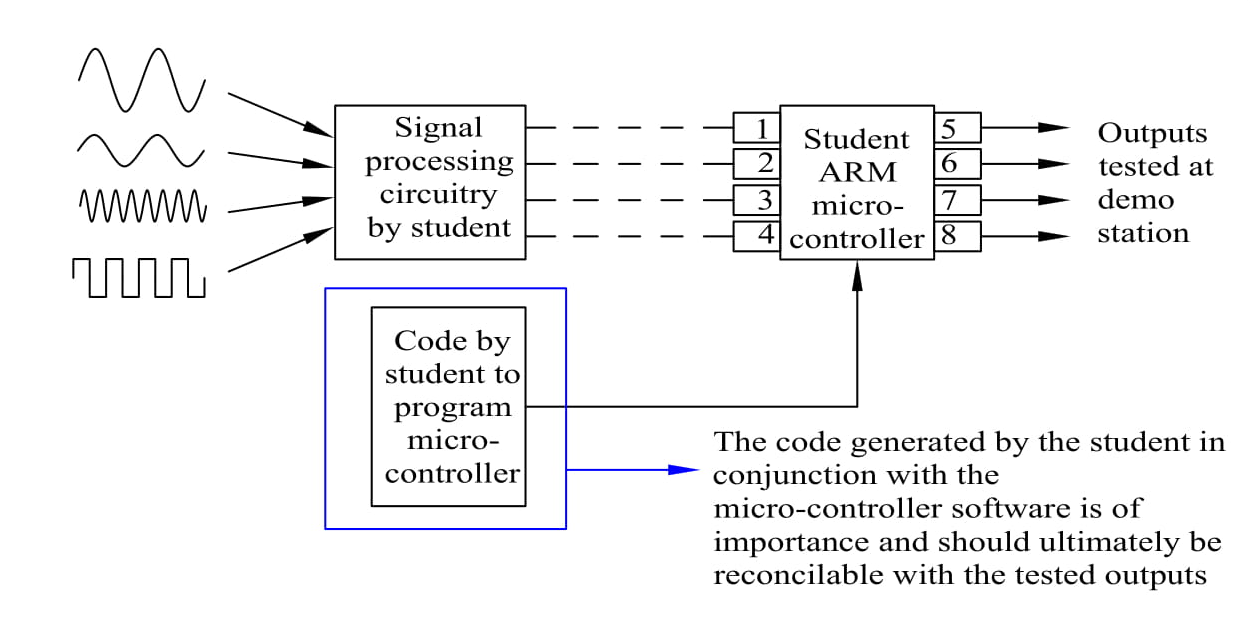
\includegraphics[width = 155mm]{diagram1.png}
\end{center}
\end{figure}
\newpage\cleardoublepage


\chapter*{2 Emulator Investigation}
\addcontentsline{toc}{chapter}{2 Emulator Investigation}
\setcounter{chapter}{2}
\setcounter{section}{0}
\setcounter{figure}{0}
\setcounter{table}{0}
\label{2emul}

\section{Emulators and Simulators}
\label{emuVsSim}
To address the problem adequately, one instruction set must be emulated on a platform compatible only with another instruction set. In this case, C code written for ARM architectures must be emulated on a \hyperref[listAbr]{PC} using CISC instruction sets.
\\\\
To achieve this, an ARM machine must be virtually created on the host machine. This can be done either through emulation or simulation. Emulation aims to mimic the target architecture (ARM) as closely as possible on the host platform (x86 Intel/AMD) at the cost of simplicity. It also provides a much less general, more platform dependent solution. In contrast, simulation aims to duplicate only high-level behaviour and is not very specific. It is not suitable for high fidelity application \cite{Chris}. The table below illustrates some key comparisons.

\begin{table}[H]
\begin{tabular}{ |c|c|c| } 
 \hline
 Goals & Emulation suitability & Simulation suitability \\ 
 \hline
 High Fidelity & Full & Partial \\ 
 Close to Real-time operation& Partial & None \\ 
 For studying principles & Partial & Full\\ 
 For recreating behavior & Full & Partial\\ 
 For general solutions & None & Full\\ 
 \hline
\end{tabular}
\caption{Emulator vs Simulators}
\label{table:1}
\end{table}

The above table illustrates the key differences in emulation and simulation and the suitability of each. As can be seen, high fidelity and operation close to real time. Only emulators are suitable. Furthermore, because behaviour is indeed being recreated and the scope has been narrowed as per \textbf{1.4 \nameref{scOfWrk}}, a simulator is not warranted. 
\\\\
It therefore becomes the goal of this investigation to find a suitable emulator for the task at hand. In the following sections emulators will be investigated. It will become apparent that these solutions are extremely specific in most cases and target a small range of \hyperref[listAbr]{MCU}s only. The choice of emulator is therefore extremely important and is precursor to automating any code evaluation.

\section{GXemul}
\label{GXemul}
The first emulator under investigation is GXemul. It is promising in that some machines using ARM processors have been emulated within its framework. Furthermore, the project is completely open-source. \cite{Gavare}
\\\\
GXemul is suitable for low-level programming courses as well as operating system courses and aims to be a learning tool more than anything else. Its framework revolves around specific machines mentioned in the pertaining documentation \cite{Gavare} \cite{gavareEmail}. Since the specific \hyperref[listAbr]{ARM} boards used in the engineering modules of importance are not supported (No Arduino or STM32 MCU support), the source-code would need to be altered to support the MCU. It is far beyond the scope of this project to code an emulators basic functioning, but it is indeed interesting that it can, theoretically be done in GXemul.
\\\\
Email correspondence with Anders Gavare (the creator of GXemul) confirmed many of the aforementioned observation and additionally provided insight into a further limitation of GXemul: It prefers host operating systems Linux and FreeBSD. Although emulation on other operating systems are indeed possible, they are not explicitly supported \cite{gavareEmail}. This makes GXemul non-ideal for the purposes of this project. It is ultimately too specific, educationally focused and lacks support for the most common platforms.
 
\section{OVPsim}
\label{OVPsim}
OVPsim provides emulation of various target architectures on multiple host platforms and includes support for multiprocessors. The OVPsim project makes use of public \hyperref[listAbr]{API}s allowing the creation of custom processors and hardware arrangements \cite{Imperas2020}. It is indeed a very versatile and complete solution.
\\\\
In contrast to GXemul, OVPsim is widely used on the most popular \hyperref[listAbr]{OS}s. This makes it suitable for the problem at hand, due to the scope being limited to Windows \hyperref[listAbr]{PC}s (with support for Linux, taking an important caveat into account)(see \textbf{1.4 \nameref{scOfWrk}}).
\\\\
Even though OVPsim seems to be suitable, very little documentation can be found regarding the process of implementing a target architecture on it. The team behind the project are not available for communication and internet forums are largely devoid of any information regarding this particular emulator. 
\\\\
A disconnect thus exists between the suitability of this emulator and the usability of it. A solution might be possible using OVPsim but there is no clear path to that solution. Further investigation into alternative emulator solutions are thus warranted.

\section{QEMU}
\label{qemu}
QEMU is a full-system emulator. It is an ubiquitous solution when it comes to \hyperref[listAbr]{ARM} processors. It is constantly being developed by the team behind it and documentation is readily available \cite{QEMU}.
\\\\
Furthermore, QEMU supports two specific \hyperref[listAbr]{ARM} Cortex-M4  \hyperref[listAbr]{MCU}s, namely the Stellaris LM3S811EVB and the Stellaris LM3S6965EVB. This makes it a very promising option, as two specific Cortex-M4 \hyperref[listAbr]{MCU}s are fully supported in terms of functionality \cite{QEMU}\cite{QEMUarm}. The previously investigated emulators, in contrast, had very little support in terms of full \hyperref[listAbr]{MCU} recreation and offered only partial solutions.
\\\\
QEMU is furthermore, a cross-platform project and therefore supports (and will continue to support for the foreseeable future) Windows \hyperref[listAbr]{PC}s. This makes it viable with the narrowing of the project scope occurring in \textbf{1.4 \nameref{scOfWrk}}. 
\\\\
It is important to note that the two ARM Cortex-M series \hyperref[listAbr]{MCU}s supported by the QEMU project are not boards usually used in the pertaining engineering modules mentioned earlier. These two boards are not aimed at low-power applications and are suited more for industrial applications than educational ones \cite{TexasInstruments2014}. Furthermore, the two boards supported by the QEMU emulator are outdated and have been superseded by the manufacturer. It becomes apparent that the QEMU emulator, in its current state, is not ideal for the purposes of this project. Indeed an emulator that supports STM32s (the \hyperref[listAbr]{MCU}s preferred for use in the pertaining engineering modules) would be preferable. Due to the fact that QEMU is open-source, it can be investigated whether these STM32 \hyperref[listAbr]{MCU}s have been implemented in projects built within the QEMU framework.

\section{The xPack Project}
\label{xpack}
The xPack Project is a modification of the the QEMU project. It modifies the open-source QEMU emulator in such a way that a wider array of Cortex-M cores are supported. This allows the emulation of various \hyperref[listAbr]{MCU}s, most notably some \hyperref[listAbr]{MCU}s in the STM32 family \cite{xPack}.
\\\\
The support, albeit partial, of the STM32 family is cardinal as ST-link`s STM32  range is the \hyperref[listAbr]{MCU} range mostly used in the pertaining engineering modules. If it can be shown that simple functionality, programmed for a real-world \hyperref[listAbr]{MCU}, can be replicated in an emulated environment, part of the problem statement as per \textbf{1.1 \nameref{ps}}, would be addressed. The real-world \hyperref[listAbr]{MCU}s available (for the aforementioned programming) are the STM32F411E and STM32F334R8-Nucleo as they were prescribed in my engineering modules and are thus in my possession.
\\\\
Since STM32 \hyperref[listAbr]{MCU}s are widely used in computer systems and design modules, an emulator that supports these boards specifically will be preferred. 
\\\\








%Whilst emulation mimics a pertaining architecture relatively closely, simulation does so more loosely. Emulation attempts to duplicate one device as accurately as possible in another environment. Simulation, by contrast, is not concerned with low-level duplication of devices, but instead mimics high-level behaviour.\cite{Chris}\newpage\cleardoublepage


\chapter*{3 System Design}
\label{system3}
\addcontentsline{toc}{chapter}{3 System Design}
\setcounter{chapter}{3}
\setcounter{section}{0}
\setcounter{figure}{0}
\setcounter{table}{0}
An autonomous system whereby C code and MCU configurations can be evaluated is needed as per \textbf{\ref{ps} \nameref{ps}}. It is standard practise for students, enrolled in the pertaining modules previously mentioned, to upload their projects as repositories (using for example GitHub). The scope of this project has been narrowed to focus on the STM32F4 family of \hyperref[listAbr]{MCU}s as per \textbf{\ref{scOfWrk} \nameref{scOfWrk}}. 
\\\\
The student repositories accessed, as part of this project, where provided by Dr Arno Barnard and are the repositories of students enrolled in E-Design 314 2020. The \hyperref[listAbr]{MCU} used, as part of this particular module in 2020, is the STM32F446RET. This implies that the \hyperref[listAbr]{MCU} was configured, programmed and debugged in STM32CubeIDE.
\\\\
In order to evaluate \hyperref[listAbr]{MCU} configurations, student code must be assessed in an autonomous way. It would be nearly impossible (and very laborious) to manually assess all the student repositories in a particular year group:

\begin{figure}[H]
\begin{center}
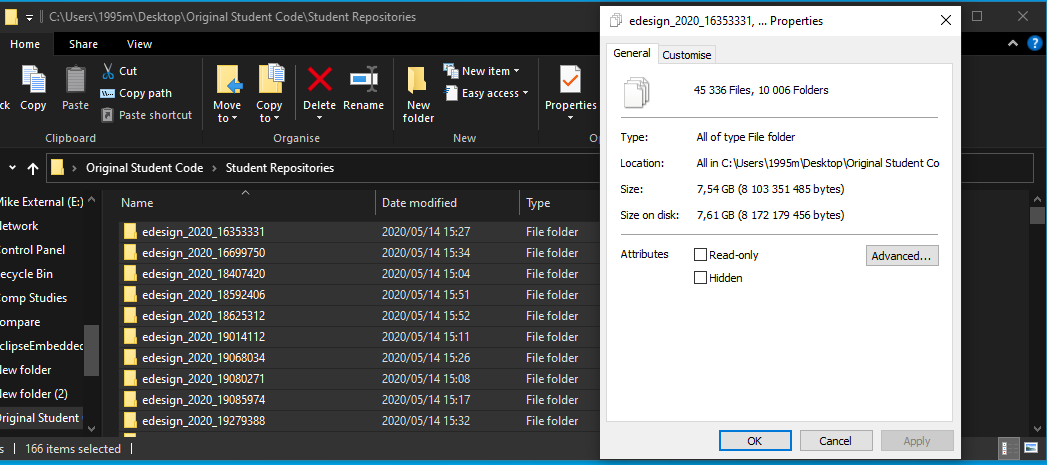
\includegraphics[width = 155mm]{misc1.png}
\caption{Student repository size}
\label{stdSize}
\end{center}
\end{figure}

Figure~\ref{stdSize} illustrates the size and number of files and folders contained within the student repositories of a single year group. It becomes readily apparent that manual code evaluation would be too laborious. An autonomous system is therefore required in order to evaluate student \hyperref[listAbr]{MCU} code.


\section{Autonomous System Outline}
\label{aso}
It has been established that student repositories are too numerous to manually navigate and evaluate. A novel solution is thus required, whereby student code can be evaluated in an autonomous way. 

\begin{figure}[H]
\begin{center}
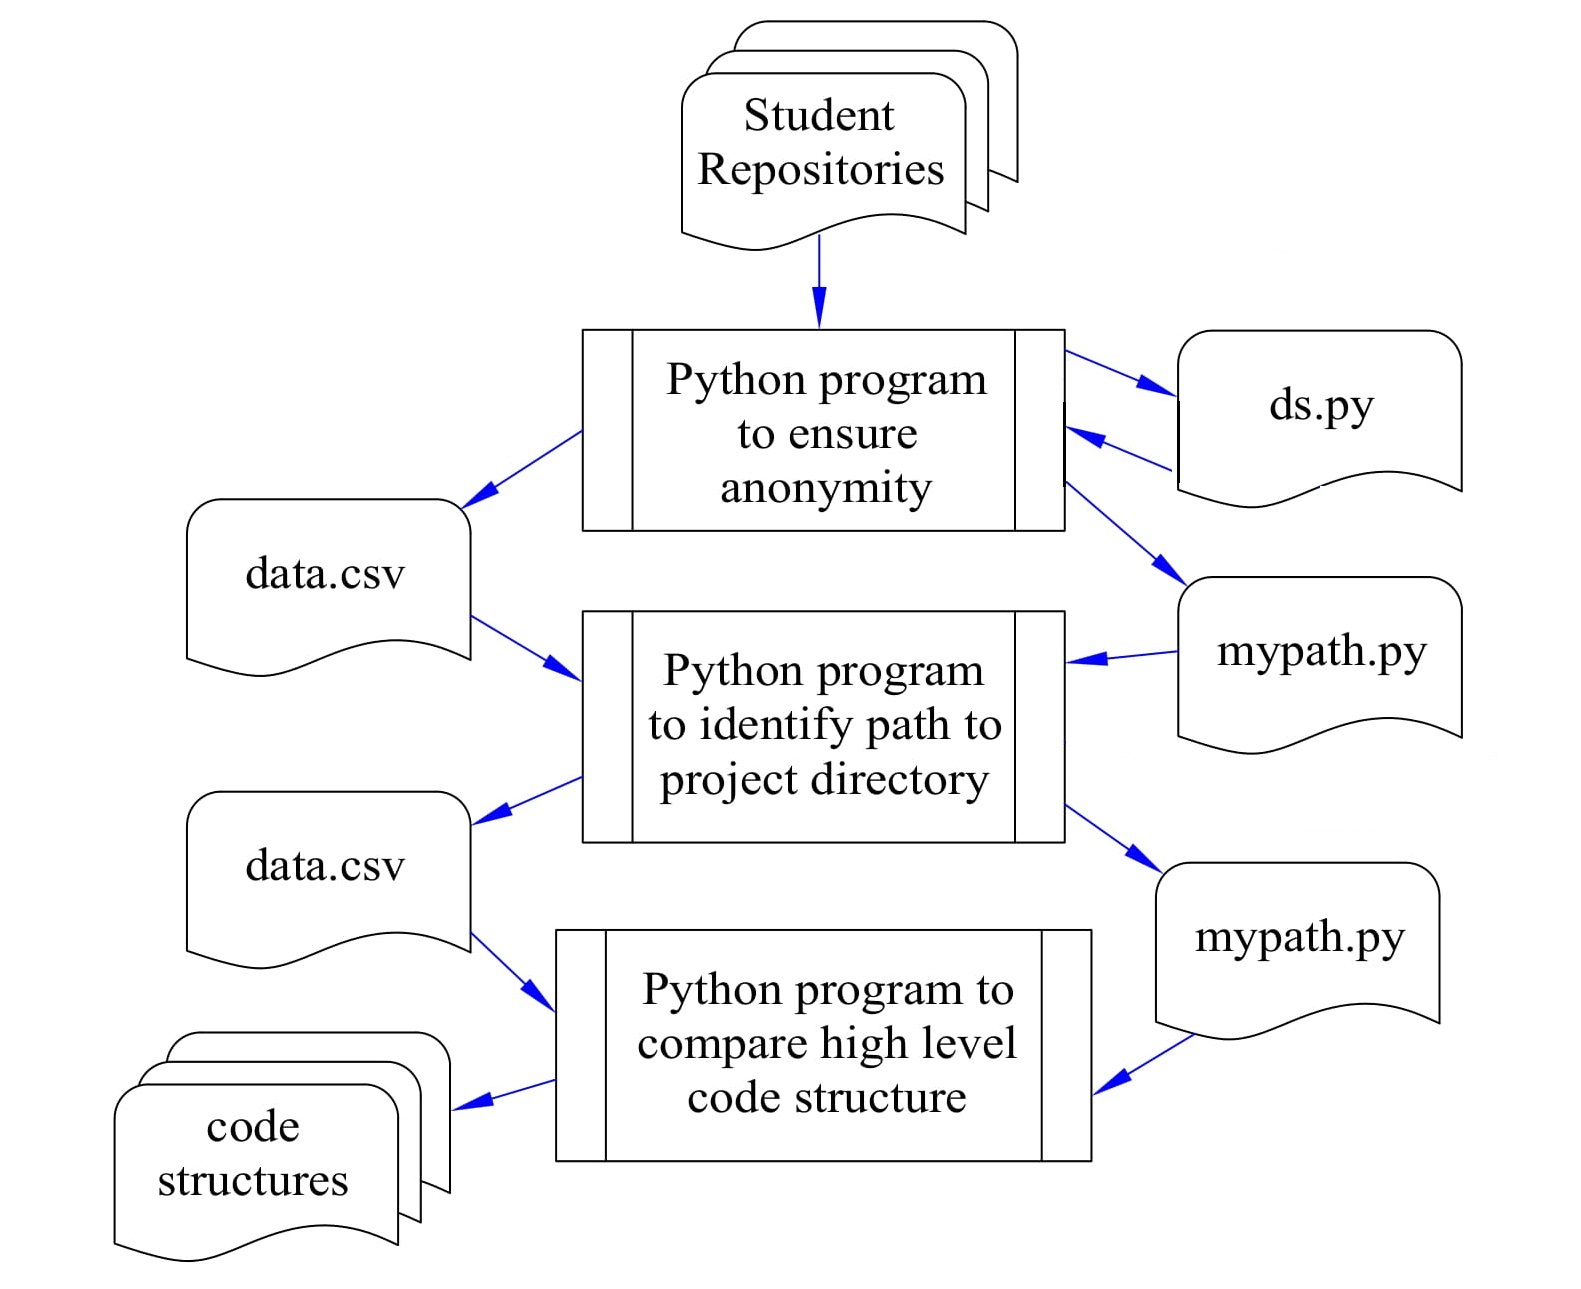
\includegraphics[width = 100mm]{flow2.jpg}
\caption{Autonomous system outline}
\label{aso}
\end{center}
\end{figure}

Figure~\ref{aso} shows the outline of the autonomous system. It can be seen that the program consists of three functional blocks and various inputs and outputs. The reasoning behind these functional block choices will briefly be discussed in the following sections. 


\subsection{Python program to ensure anonymity}
\label{p1}

STM32CubeIDE has a very particular project structure consisting of various directories containing source code, included libraries, drivers and debugger files. These directories are contained within a project root directory and the general structure is highlighted below:

\begin{figure}[H]
\begin{center}
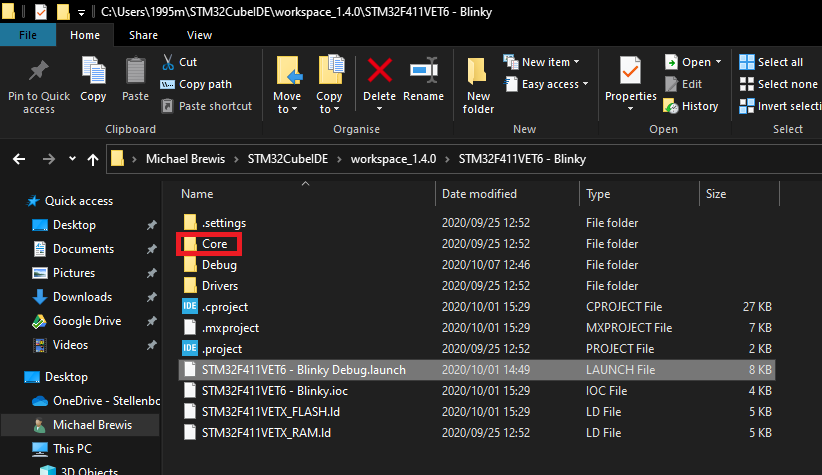
\includegraphics[width = 120mm]{stmProject.png}
\caption{STM32CubeIDE project structure}
\label{stmProj}
\end{center}
\end{figure}

Figure~\ref{stmProj} illustrates the default STM32CubeIDE project outline. It can be seen that any valid project contains a "Core" folder. This folder contains all the relevant C code and included libraries. It is this folder that is of relevance. The project illustrated above was created in STM32CubeIDE to blink an LED on an STM32F411 \hyperref[listAbr]{MCU}. It is, however, not part of the repositories sent by Dr A Barnard. These repositories are, in fact, not depicted in order to maintain student anonymity. 
\\\\
Anonymity is indeed a very important part of the automation process, when it comes to evaluating student code. Once access to the repositories have been gained, it becomes necessary to remove student numbers from folder and file names. The ethical reason for this is twofold. Firstly, students submit their respective repositories without opting into its use as part of this project. Secondly, this project does not aim to identify cases of plagiarism. If a case of plagiarism is identified as a side effect of the autonomous system, it is vital that these cases cannot be traced back to students.
\\\\
It can be seen that there is only one input to the relevant python script. This input is all the relevant student repositories. How the autonomous system identifies these repositories and interacts with them will be discussed in \textbf{\nameref{4detailedd}}.
\\\\
It can be observed from Figure~\ref{aso}, that the python script which ensures anonymity has three outputs. The first output is another python script called ds\hyperref[listExt]{.py} which stores random unique identifiers associated with specific student numbers. As a result the ds\hyperref[listExt]{.py} file generated can be imported by second executions of this program in order to populate the needed Pandas Data Frame. A second file, namely mypath\hyperref[listExt]{.py}, is also generated. This file is used to store the absolute path of certain directories and files within the project root directory and will be discussed in greater detail in \textbf{\nameref{4detailedd}}. Lastly, the third output is the data\hyperref[listExt]{.csv} file. It is generated within the first script and populated using the ds\hyperref[listExt]{.py} module.

\subsection{Python program to identify path to project directories}
\label{p2}
Once the needed outputs, from the first program, as per Figure~\ref{aso} have been generated, a python program is needed to save the absolute path to the relevant folder within each student repository. This will ensure that the python programs work on any PC and are not relative to the folder hierarchies of the host machine. The absolute path to the needed folders will indeed serve as input to the rest of the programs in the autonomous system depicted in Figure~\ref{aso}.
\\\\
Although it is not immediately apparent that this functional block is prominent enough to be conceptualized as a separate program, this is not the case. The identification of the relevant folder (and contained files) is a cardinal step in the autonomous system. This is because students often submit their projects in such a way, that the project folder is nested within various parent directories. If the rest of the autonomous system is to function correctly, the project directory must be identified and its absolute path stored. Moreover, the aforementioned functionality should be maintained regardless of multiple nested directories.
\\\\
It can be seen form Figure~\ref{aso} that the functional block discussed in this subsection receives, as inputs, the outputs generated by the program discussed in \textbf{\ref{p1} \nameref{p1}}. Firstly, the mypath\hyperref[listExt]{.py} module is needed to navigate the folder directories on the host machine as saved by the first program. Next, the data\hyperref[listExt]{.csv} file is required to link student repositories with unique identifiers as assigned by the first program. This file will, additionally, be modified by the program discussed in this subsection, to store the absolute path to the pertaining project folder.  

\subsection{Python program to evaluate high-level code structures}
\label{p3}

The final program in the execution chain of the autonomous process creates files for comparison. It receives the outputs of the previous python programs. The function of this step in the autonomous process, is to identify and extract student created configurations, both in STM32CubeIDE created files as well as the students main\hyperref[listAbr]{.c} file.
\\\\
To begin with, this program will receive the data\hyperref[listExt]{.csv} file (modified by previous steps in the automation process). The data\hyperref[listExt]{.csv} file, at this point, will contain all the needed paths to student specific project repositories on the host machine. It is, moreover, required to assure that repositories are valid and that student numbers have been linked to unique identifiers. This program will, furthermore after execution, delete the data\hyperref[listExt]{.csv} file to ensure that students are not implicated in cases of plagiarism. The ethical reasons for this are discussed in \textbf{\ref{p1} \nameref{p1}}. The aforementioned functionality can easily be omitted if cases of plagiarism are indeed to be detected. 
\\\\
In addition to the data\hyperref[listExt]{.csv} file, this program also receives, as input, the mypath\hyperref[listExt]{.py} module. This is, once again, needed in order to produce the outputs of the program in the correct directory on the host PC.

\subsection{Autonomous process directory structure}
\label{p4}
In the previous subsections, the autonomous process has been outlined. The outputs produced by each of the steps in this process have also been discussed. This subsection will highlight the folder structure produced and utilized by the relevant system. Due to the modular nature of the autonomous system, the outputs of one process are often the inputs to another. Furthermore, the programs have been written in such a way that multiple executions of a single process are often necessitated.
\\\\
It therefore, becomes necessary to store these outputs and inputs in a common directory, to be accessed by any iteration of the various steps in the process. The figure below illustrates these directories.

\begin{figure}[H]
\begin{center}
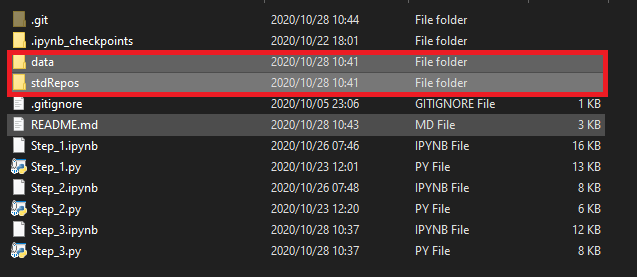
\includegraphics[width = 100mm]{dir.png}
\caption{Pertaining autonomous process directories}
\label{dir}
\end{center}
\end{figure}

Figure~\ref{dir} illustrates the two directories produced by the autonomous process. This will be discussed in greater detail in \textbf{\ref{step1} \nameref{step1}}. It can be seen from the figure that "stdRepos" and "data" are produced as two directories. Within the "stdRepos" directory, the various student repositories are to be placed by the user of the host machine. The subsequent steps in the autonomous process will access the "stdRepos" directory and the various nested folders within. These nested folders are depicted in the following figure:

\begin{figure}[H]
\begin{center}
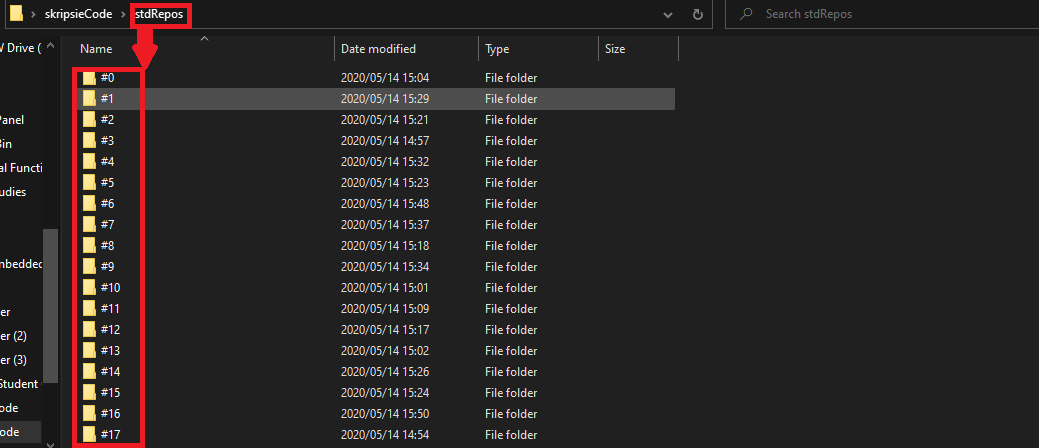
\includegraphics[width = 140mm]{stdRepos.png}
\caption{Content of the stdRepos folder}
\label{stdRepos12}
\end{center}
\end{figure}

Figure~\ref{stdRepos12} depicts the content of the "stdRepos" folder, after the program discussed in \textbf{\ref{p1} \nameref{p1}}, has executed.
\\\\
In addition to the previously discussed repository a "data" repository is also created by the process in discussion. This repository will serve as a common storage location for any programs that form part of the system. Within this directory the output files of the final step are stored, as well as the required python modules created by the system. The contents of the "data" folder are partially displayed in the following figure:

\begin{figure}[H]
\begin{center}
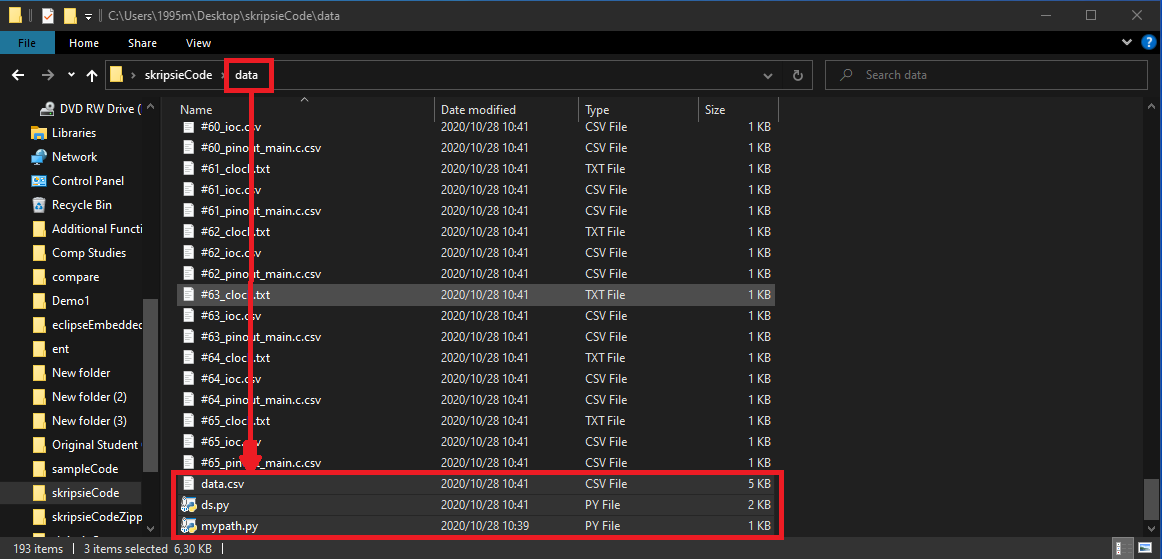
\includegraphics[width = 155mm]{data.png} 
\caption{Content of the data folder}
\label{data23}
\end{center}
\end{figure}

Figure ~\ref{data23} depicts the content of the data folder, after all the programs discussed in \textbf{\ref{aso} \nameref{aso}}, have executed. It can be seen that the pertaining python modules (namely mypath\hyperref[listExt]{.py} and ds\hyperref[listExt]{.py}) as well as the data\hyperref[listExt]{.csv} is contained within this repository. In addition to these files, the various student structures are also stored in this folder as illustrated in \textbf{\ref{3res} \nameref{3res}}. The various functional blocks depicted in Figure~\ref{stdRepos}, will have access to the respective directories using the mypath\hyperref[listExt]{.py} module in the "data" directory.
\\\\
This subsection concludes the outline of the autonomous system and provides a general overview of the system. In the following chapter each of the functional blocks discussed in \textbf{\ref{p1} \nameref{p1}}, \textbf{\ref{p2} \nameref{p2}} and \textbf{\ref{p3} \nameref{p3}} will be expanded upon.
\newpage\cleardoublepage


\chapter*{4 Detailed Design}
\label{4detailedd}
\addcontentsline{toc}{chapter}{4 Detailed Design}
\setcounter{chapter}{4}
\setcounter{section}{0}
\setcounter{figure}{0}
\setcounter{table}{0}

In \textbf{\nameref{3}}, a general overview of the autonomous system (created in order to evaluate high-level code structures) was given. This chapter will expand upon the concepts and functions introduced in \textbf{\nameref{3}}. It will, furthermore, outline the python modules required by the various programs and outline why they are dependencies. Lastly, this chapter will outline the process required in order to create Windows \hyperref[listExt]{.exe} files for the three step autonomous system. 

\section{Python dependencies}
\label{PyDep}

\section{Detailed design}
\label{detDes}

In this section the information provided in \textbf{\ref{aso} \nameref{aso}} will be elaborated upon. For each functional block in Figure~\ref{aso} a flow diagram of the program logic will be presented. Each functional block will be discussed in detail thereafter. A caveat to the aforementioned, is that not all the lines of code that make up the system will be described. This decision was made for the sake of conciseness. The entirety of the system code can, however, be viewed in \textbf{\nameref{C}}, \textbf{\nameref{D}} and \textbf{\nameref{E}}.
\\\\
Lastly, some of the critical functions of the autonomous process are nested in other functions. They will thus be discussed within the context of the functional block in which they are nested. An example of this is the creation of the "data" directory, within the creation of the ds.py module as seen in \textbf{\ref{mypath} \nameref{mypath}}.

\newpage\cleardoublepage

\subsection{Step1.py}
\label{step1}

The figures below depict the logical flow of the first python program as discussed and depicted in \textbf{\ref{p1} \nameref{p1}}. 
\begin{figure}[H]
\begin{center}
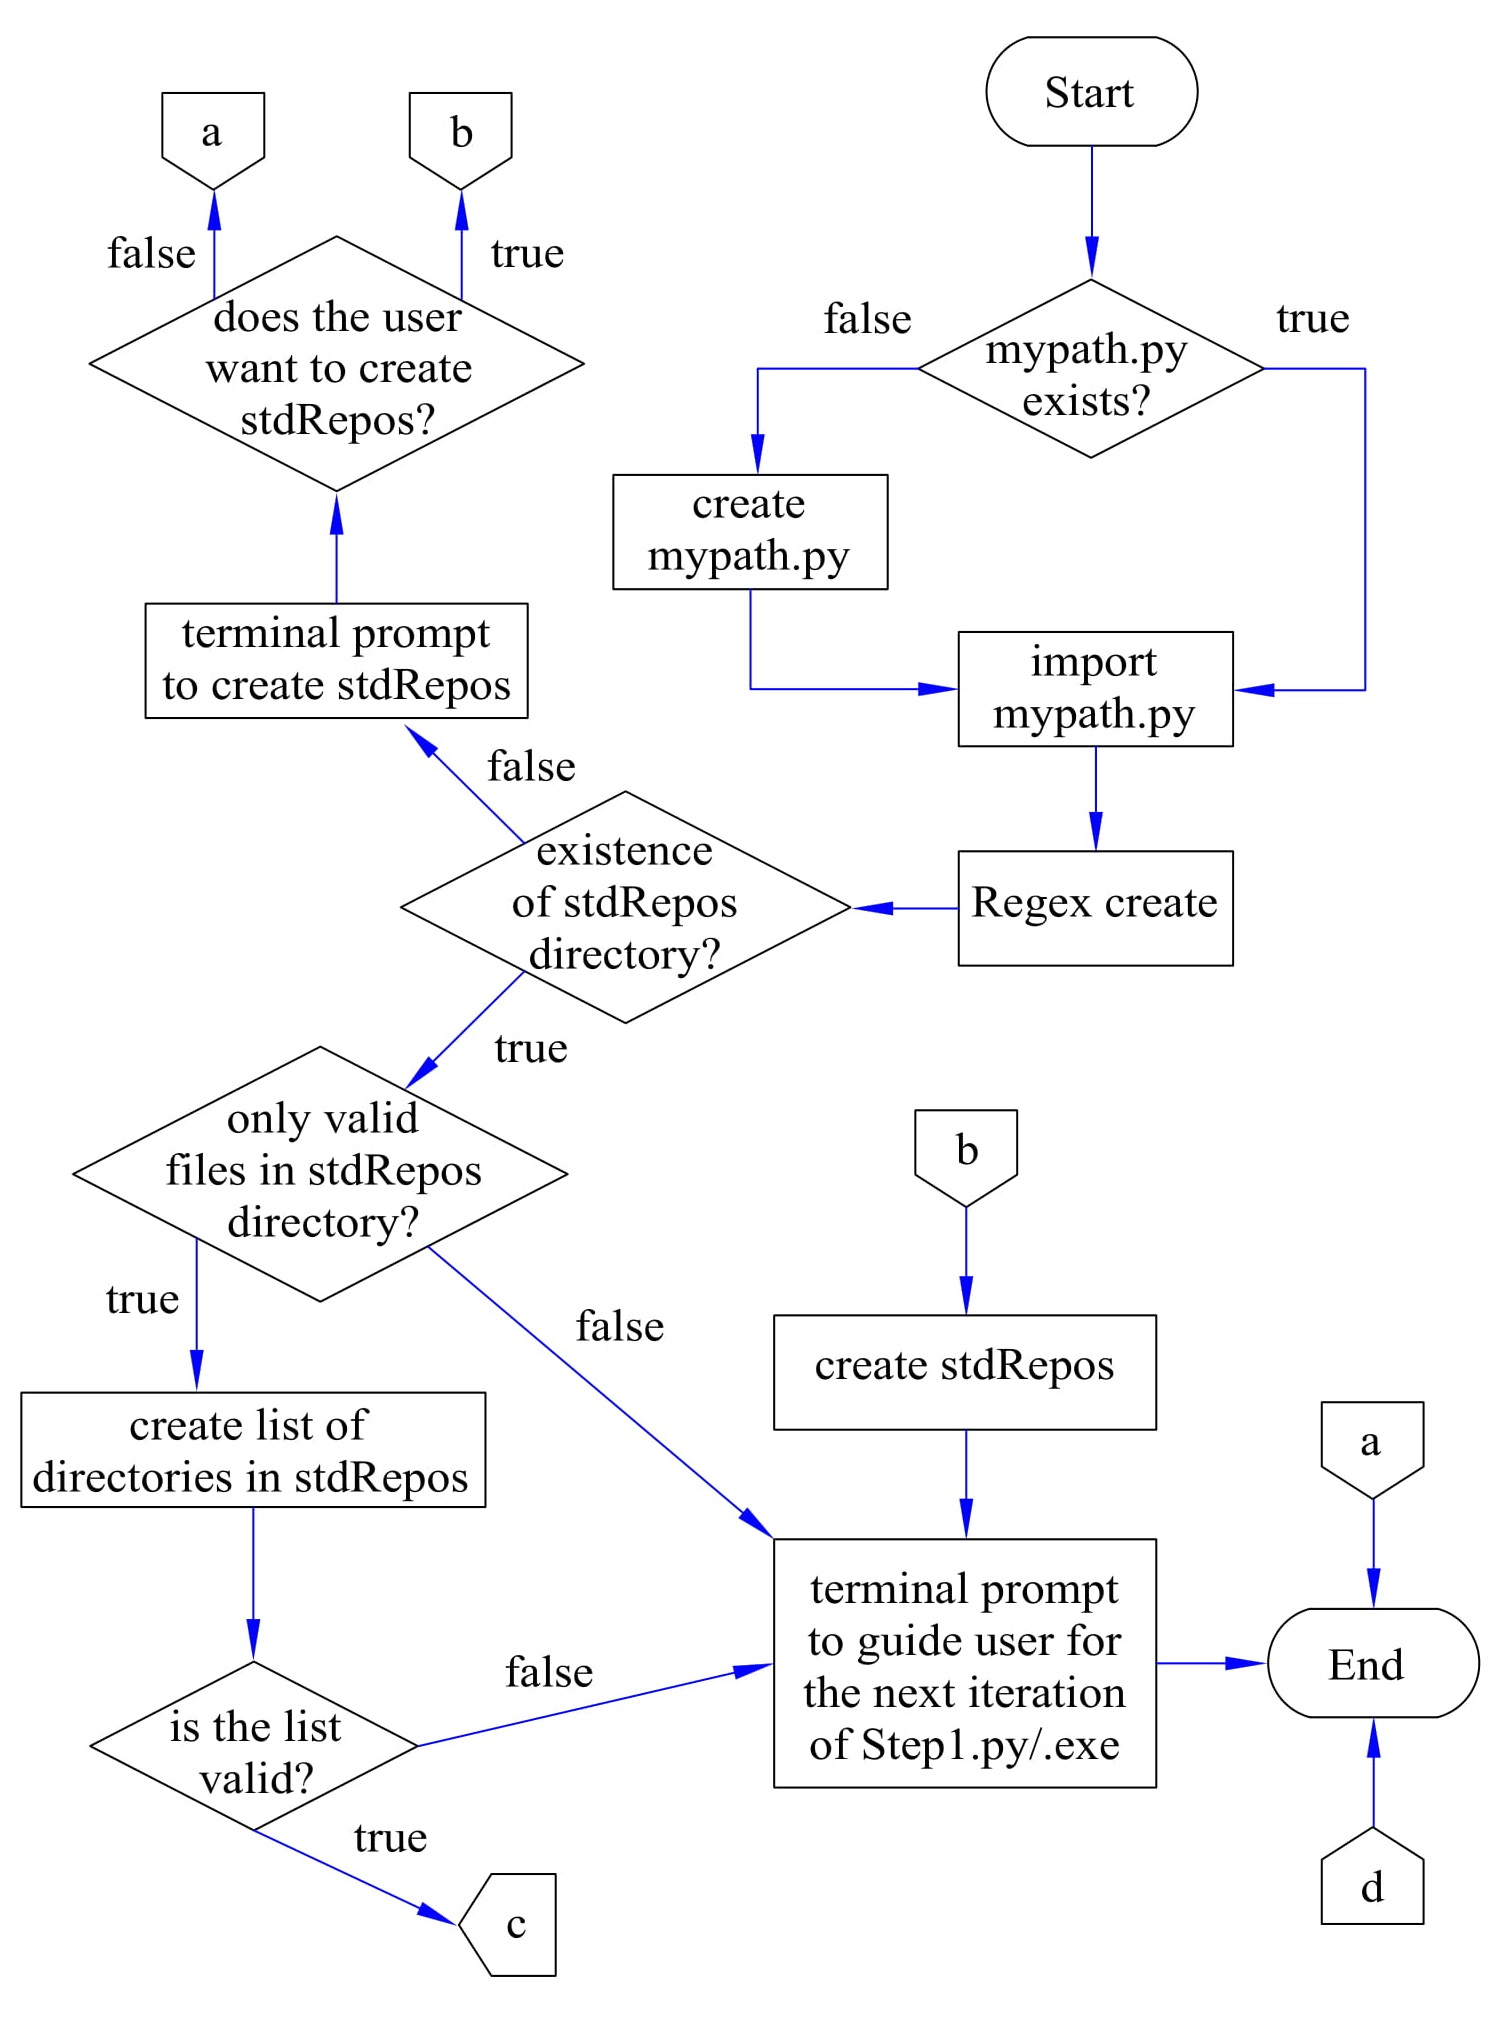
\includegraphics[width = 155mm]{1.1.jpg}
\caption{Step1 flow diagram 1}
\label{1.1}
\end{center}
\end{figure}

\begin{figure}[H]
\begin{center}
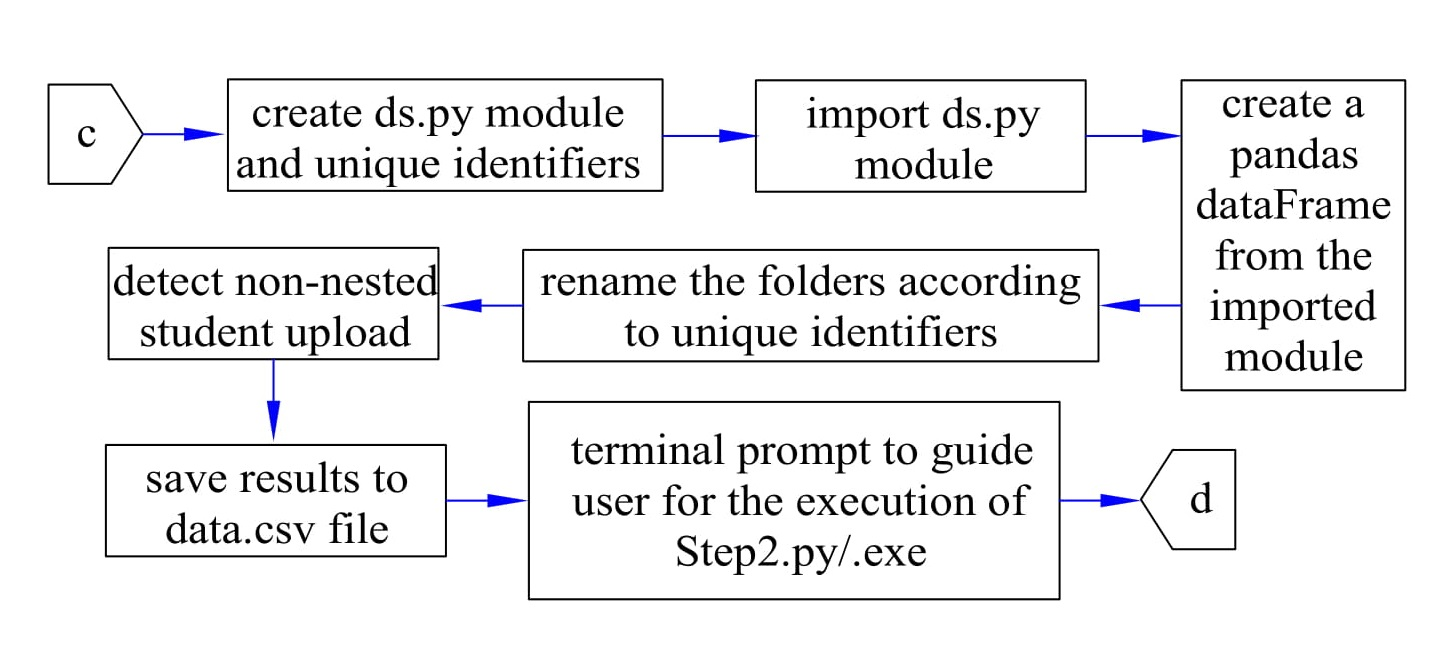
\includegraphics[width = 155mm]{1.2.jpg}
\caption{Step1 flow diagram 2}
\label{1.2}
\end{center}
\end{figure}

As can be see in Figure~\ref{1.1} and Figure~\ref{1.2}, the logical parts of the Step1.py/.exe are quite extensive and will only partially be discussed. 

\subsubsection{mypath.py module}
\label{mypath}

The various programs that comprise the autonomous system will be executed on a host PC other than the one they were created on. Since the user of the host PC can place the autonomous system (consisting of three programs) anywhere in the file system of the aforementioned PC, identifying the root repository becomes necessary. It is indeed important, that the programs in the autonomous chain, are able to execute regardless of where in the host file system they are located. 
\\\\
Regarding the above observation, it was decided that a python module is to be created in order to save the home, "stdRepos" and "data" directories. The code snippet below illustrates the process of creating the "data" directory as well as the mypath.py module. It further illustrates how the aforementioned module is imported into the program after creation.
\\\\
\lstinputlisting[label={code1},caption={mypath.py and data folder creation and import}, language=Python]{code1.py}

It can be seen from Listing~\ref{code1}: lines 13 - 24 that the program will create a "data" directory within the home directory (where the programs are located). In addition to the creation of this directory, a module is created and stored within the "data" directory, namely mypath.py \cite{Sweigart2015}.
\\\\
It is of note, that the aforementioned functionality strictly occurs if the "data" directory and the mypath.py module does not yet exist. If these entities do however exist, the module is simply imported as per  Listing~\ref{code1}: lines 5 - 11. Since Step1.py/.exe is created with multiple executions in mind, the decision was taken to use the above discussed approach.

\begin{figure}[H]
\begin{center}
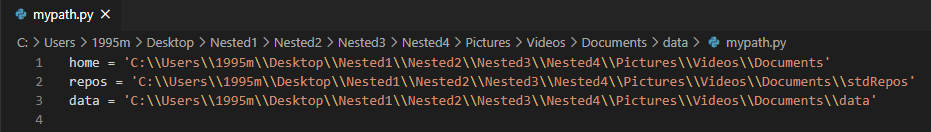
\includegraphics[width = 155mm]{mypath.pyCon.png}
\caption{mypath.py module content}
\label{mypath.pyCon}
\end{center}
\end{figure}

Figure~\ref{mypath.pyCon} illustrated the content of the pertaining module. Moreover, it illustrates how the directories of importance are stored regardless of location within a file system. The absolute path to the various directories are saved to be utilized by subsequent executions of Step1.py/.exe, in addition to the other programs in the autonomous chain.


\subsubsection{Regex creation}
\label{regex1}
As indicated in \textbf{\ref{p1} \nameref{p1}}, an important requisite of the autonomous process is the introduction of anonymity. It is, in fact, necessary to remove and replace all instances of student numbers from directory and file names for reasons mentioned in \textbf{\nameref{3}}. In order to facilitate the fulfilment of anonymity, it was decided to introduce regular expressions to the various programs in the autonomous system. These regular expressions are henceforth abbreviated simply as regex. 

\lstinputlisting[label={code2},caption={Regex initialization}, language=Python]{code2.py}

Listing~\ref{code2} depicts the regular expressions introduced as part of Step1.py/.exe. Lines 1-3 are simply regular expressions used to identify different variants of student numbers \cite{Sweigart2015}\cite{regex}. Line 4 consists of a regex pattern used to identify a valid student number unique identifier and will be expanded upon in \color{green}that part \color{black}.
\subsubsection{stdRepos directory}
\label{stdRepos}
\lstinputlisting[label={code3},caption={Regex initialization}, language=Python]{code3.py}

Listing~\ref{code3} depicts the code written to:
\\\\
\begin{enumerate}
\item Detect the existence of the "stdRepos" directory.
\item Create the "stdRepos" directory if the user so wishes.
\item Detect valid repositories within the "stdRepos" directory.
\item Create and handle all command prompts associated with the above mentioned functionality.
\end{enumerate}

It can be seen from Listing~\ref{code3}: Lines 1-21, that the program will test for the existence of the "stdRepos" folder within the home directory. If this directory is not detected, a command prompt will be displayed giving the user the option to create the "stdRepos" folder in the correct location. Thereafter, the program will exist after prompting the user to rerun Step1.py/.exe.
\\\\
It is assumed that the user will extract any student repositories within the "stdRepos" folder. It can be seen from Listing~\ref{code3}: Line 24, that the regex mentioned in \textbf{\ref{regex1} \nameref{regex1}}, is applied to the directory names within the "stdRepos" folder. If a match is detected a list is populated with the matched string. This list will be used in future functional blocks. 
\\\\
It can, lastly, be seen that any invalid files in the "stdRepos" folder will also be detected by the program. If indeed a folder/file is located within the directory but is not matched by a student number detection regex or a unique identifier regex, a command prompt will guide the user in the next step. The aforementioned functionality is depicted in Listing~\ref{code3}: Lines 27-40.

\subsubsection{ds.py module}
\label{ds}
\begin{figure}[H]
\begin{center}
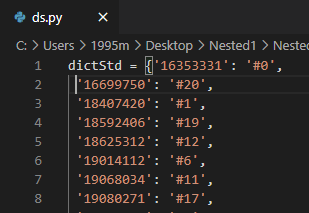
\includegraphics[width = 50mm]{ds.py.png}
\caption{ds.py module content}
\label{ds.pyCon}
\end{center}
\end{figure}

Figure~\ref{ds.pyCon} displays the content of the ds.py module. It depicts the linking of unique identifiers with student numbers. It is important to note that anonymity is not compromised by the ds.py module as it is deleted after the autonomous process finishes. Furthermore, each iteration of Step1.py/.exe randomly assigns unique identifiers to student numbers and the identifiers depicted in Figure~\ref{ds.pyCon}, will change from iteration to iteration. 

\lstinputlisting[label={code4},caption={ds.py creation}, language=Python]{code4.py}

Listing~\ref{code4}: Lines 1-12 depicts the code written to create a dictionary based on the content of the "stdRepos" folder. Randomly produce indexes are linked to student numbers and stored in a dictionary. It furthermore, illustrates (lines 14-24) how the mentioned dictionary is stored as a python module to be imported and utilized by the other steps in the autonomous process. 

\subsubsection{Pandas DataFrame}
\label{datFra}
It was decided to use a Pandas Data Frame to store any information extracted from student repositories. A Pandas Data Frame was selected above similar frameworks due to the ease with which data in the frame can be manipulated and searched. In order to populate the Pandas Data Frame, the previously created ds.py module must be imported by the program. This is all done in a very straight forward and standard way and will thus not be expanded upon.  


\subsubsection{Rename the folders}
\label{renFol}
\lstinputlisting[label={code5},caption={Folder renaming}, language=Python]{code5.py}

In Listing~\ref{code5}: lines 1-12, it can be observed that the folders within the "stdRepos" directory are renamed using a nested for-loop. The first for-loop iterates through all the folders within the "stdRepos" directory. The second (nested) for-loop, loops through the Pandas Data Frame (populated with unique identifiers linked to student numbers) and renames the current folder (the subject of the first for-loop) to the linked unique identifier.
\\\\
In short, for each folder in the "stdRepos" directory the Pandas Data Frame is looped to find the specific unique identifier associated with the pertaining folder student number. The folders are then renamed according to the identifier. 


\subsubsection{data.csv file}
\label{data.csv}
Lastly, the previously mentioned Pandas Data Frame is stored as data.csv in the "data" directory. This file (data.csv) will be used to facilitate the population of Pandas Data Frames used by the subsequent steps in the automation process. 



\subsection{Step2.py}
\label{step2}

\begin{figure}[H]
\begin{center}
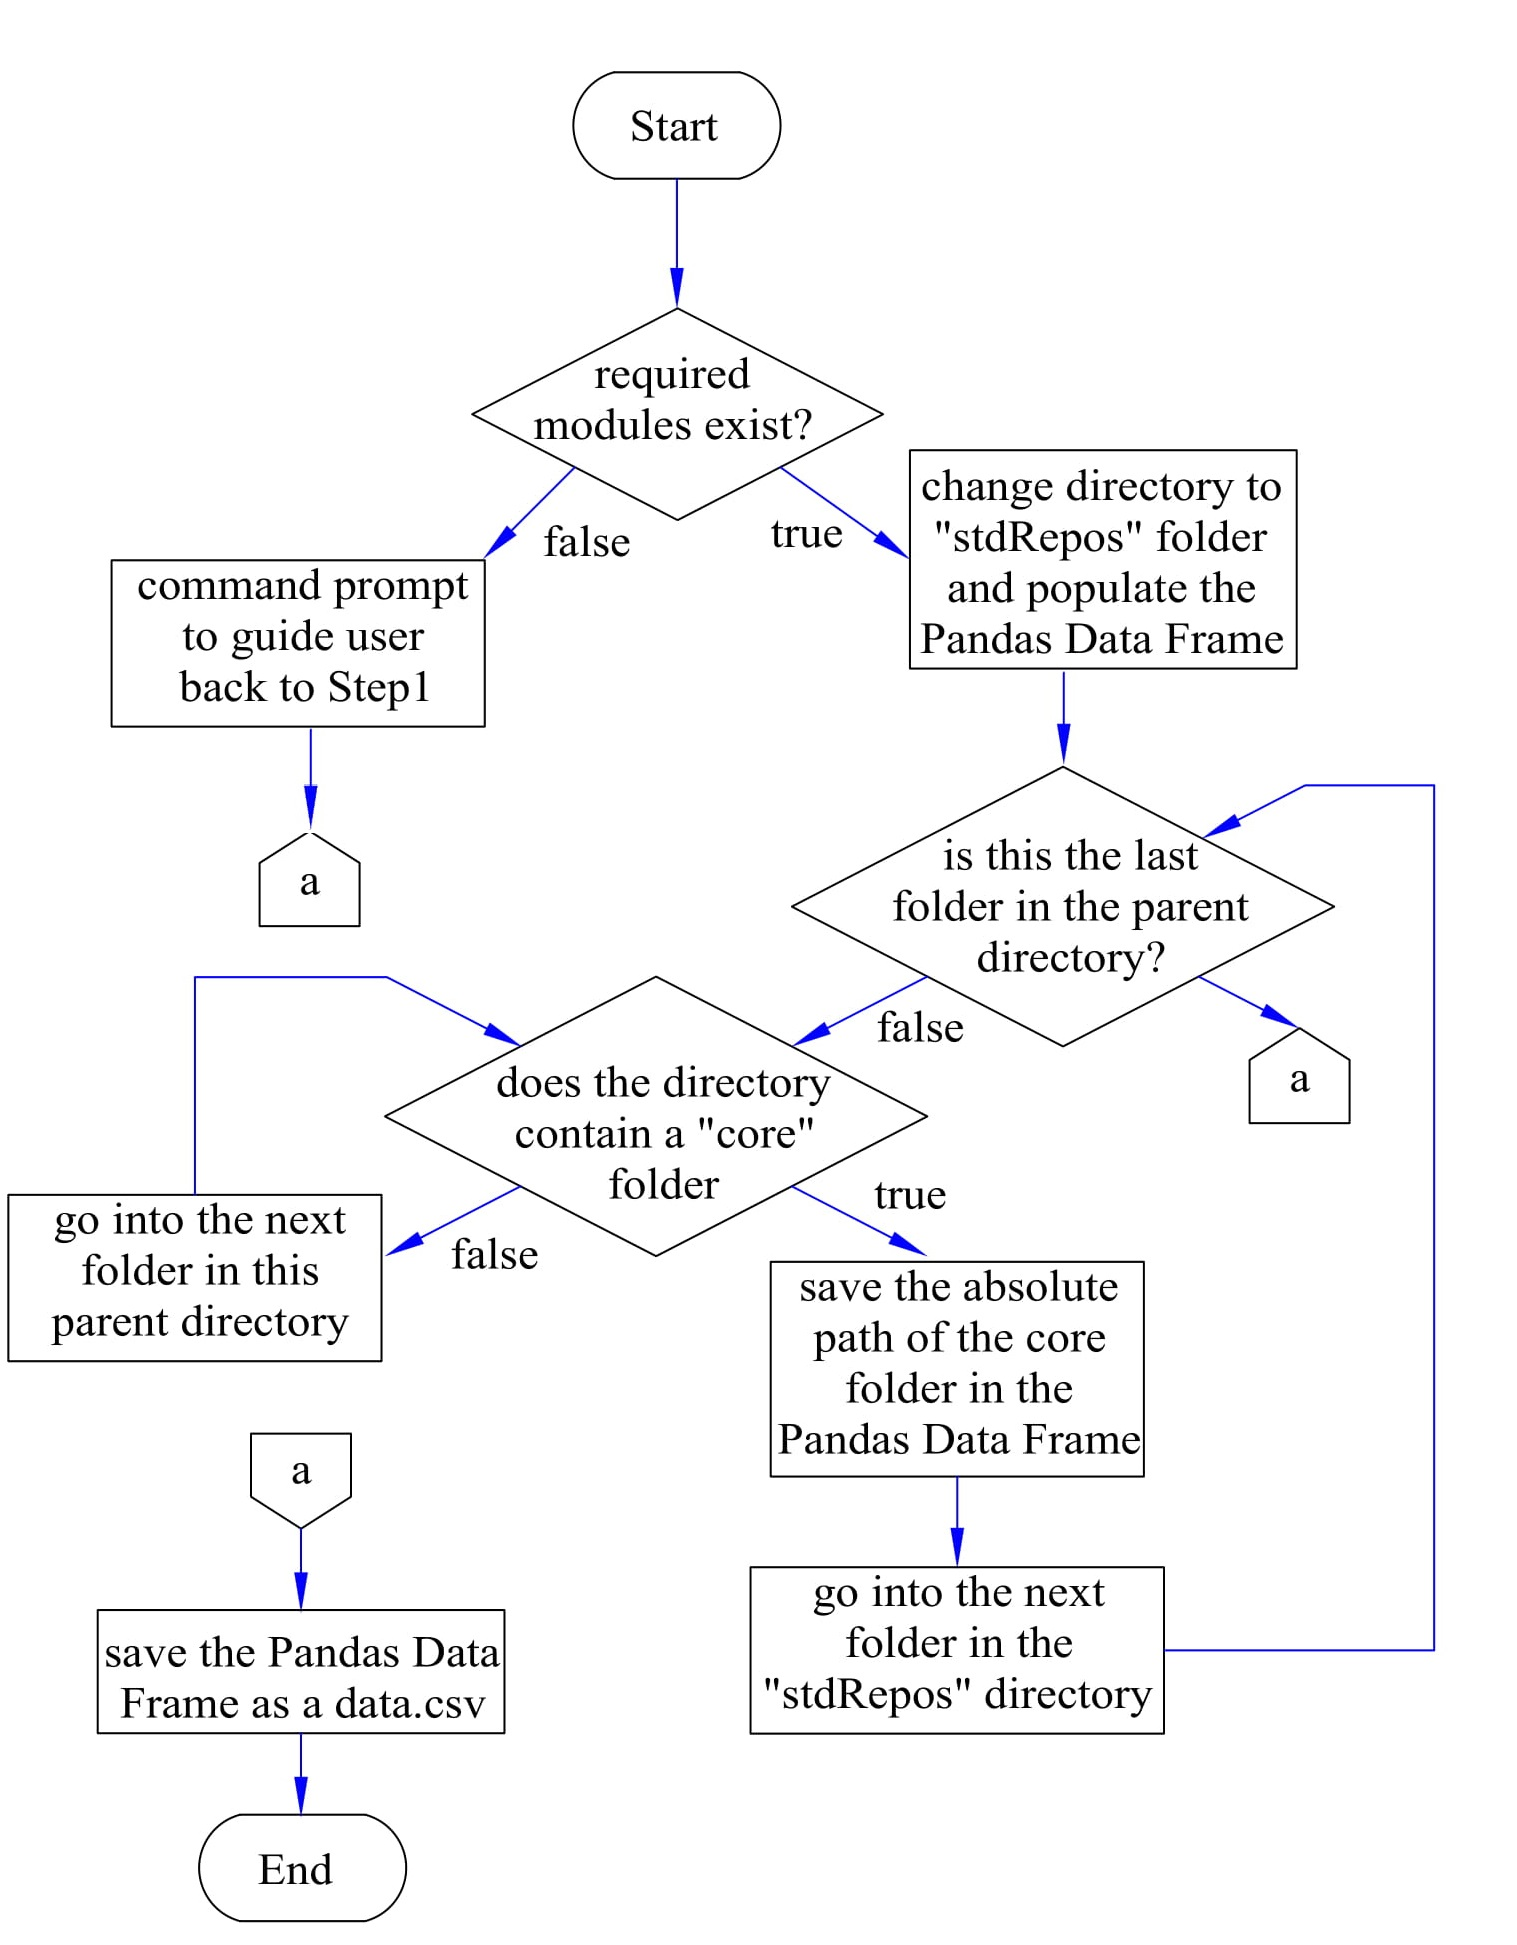
\includegraphics[width = 155mm]{2.jpg}
\caption{Step2 flow diagram}
\label{2}
\end{center}
\end{figure}

\subsection{Step3.py}
\label{step3}

\section{Windows executable files}
\label{exe}
\newpage\cleardoublepage


\chapter*{5 Results}
\label{results}
\addcontentsline{toc}{chapter}{5 Results}
\setcounter{chapter}{5}
\setcounter{section}{0}
\setcounter{figure}{0}
\setcounter{table}{0}

In this chapter the results of the autonomous system will be illustrated and discussed. Due to the two-part nature of the problem at hand, the results will be presented in accordance. 

\section{Emulation results} 
\label{emuRes}
This section will detail the results obtained, when attempting to introduce basic LED flashing functionality, on the emulator as described in \textbf{\nameref{2emul}}. Firstly, it will be shown how the aforementioned functionality is achieved on a real-world MCU. Thereafter, the mentioned functionality will be demonstrated in an emulated environment.
\subsection{Real world MCU in STM32CubeIDE}
\label{real}

\begin{figure}[H]
\begin{center}
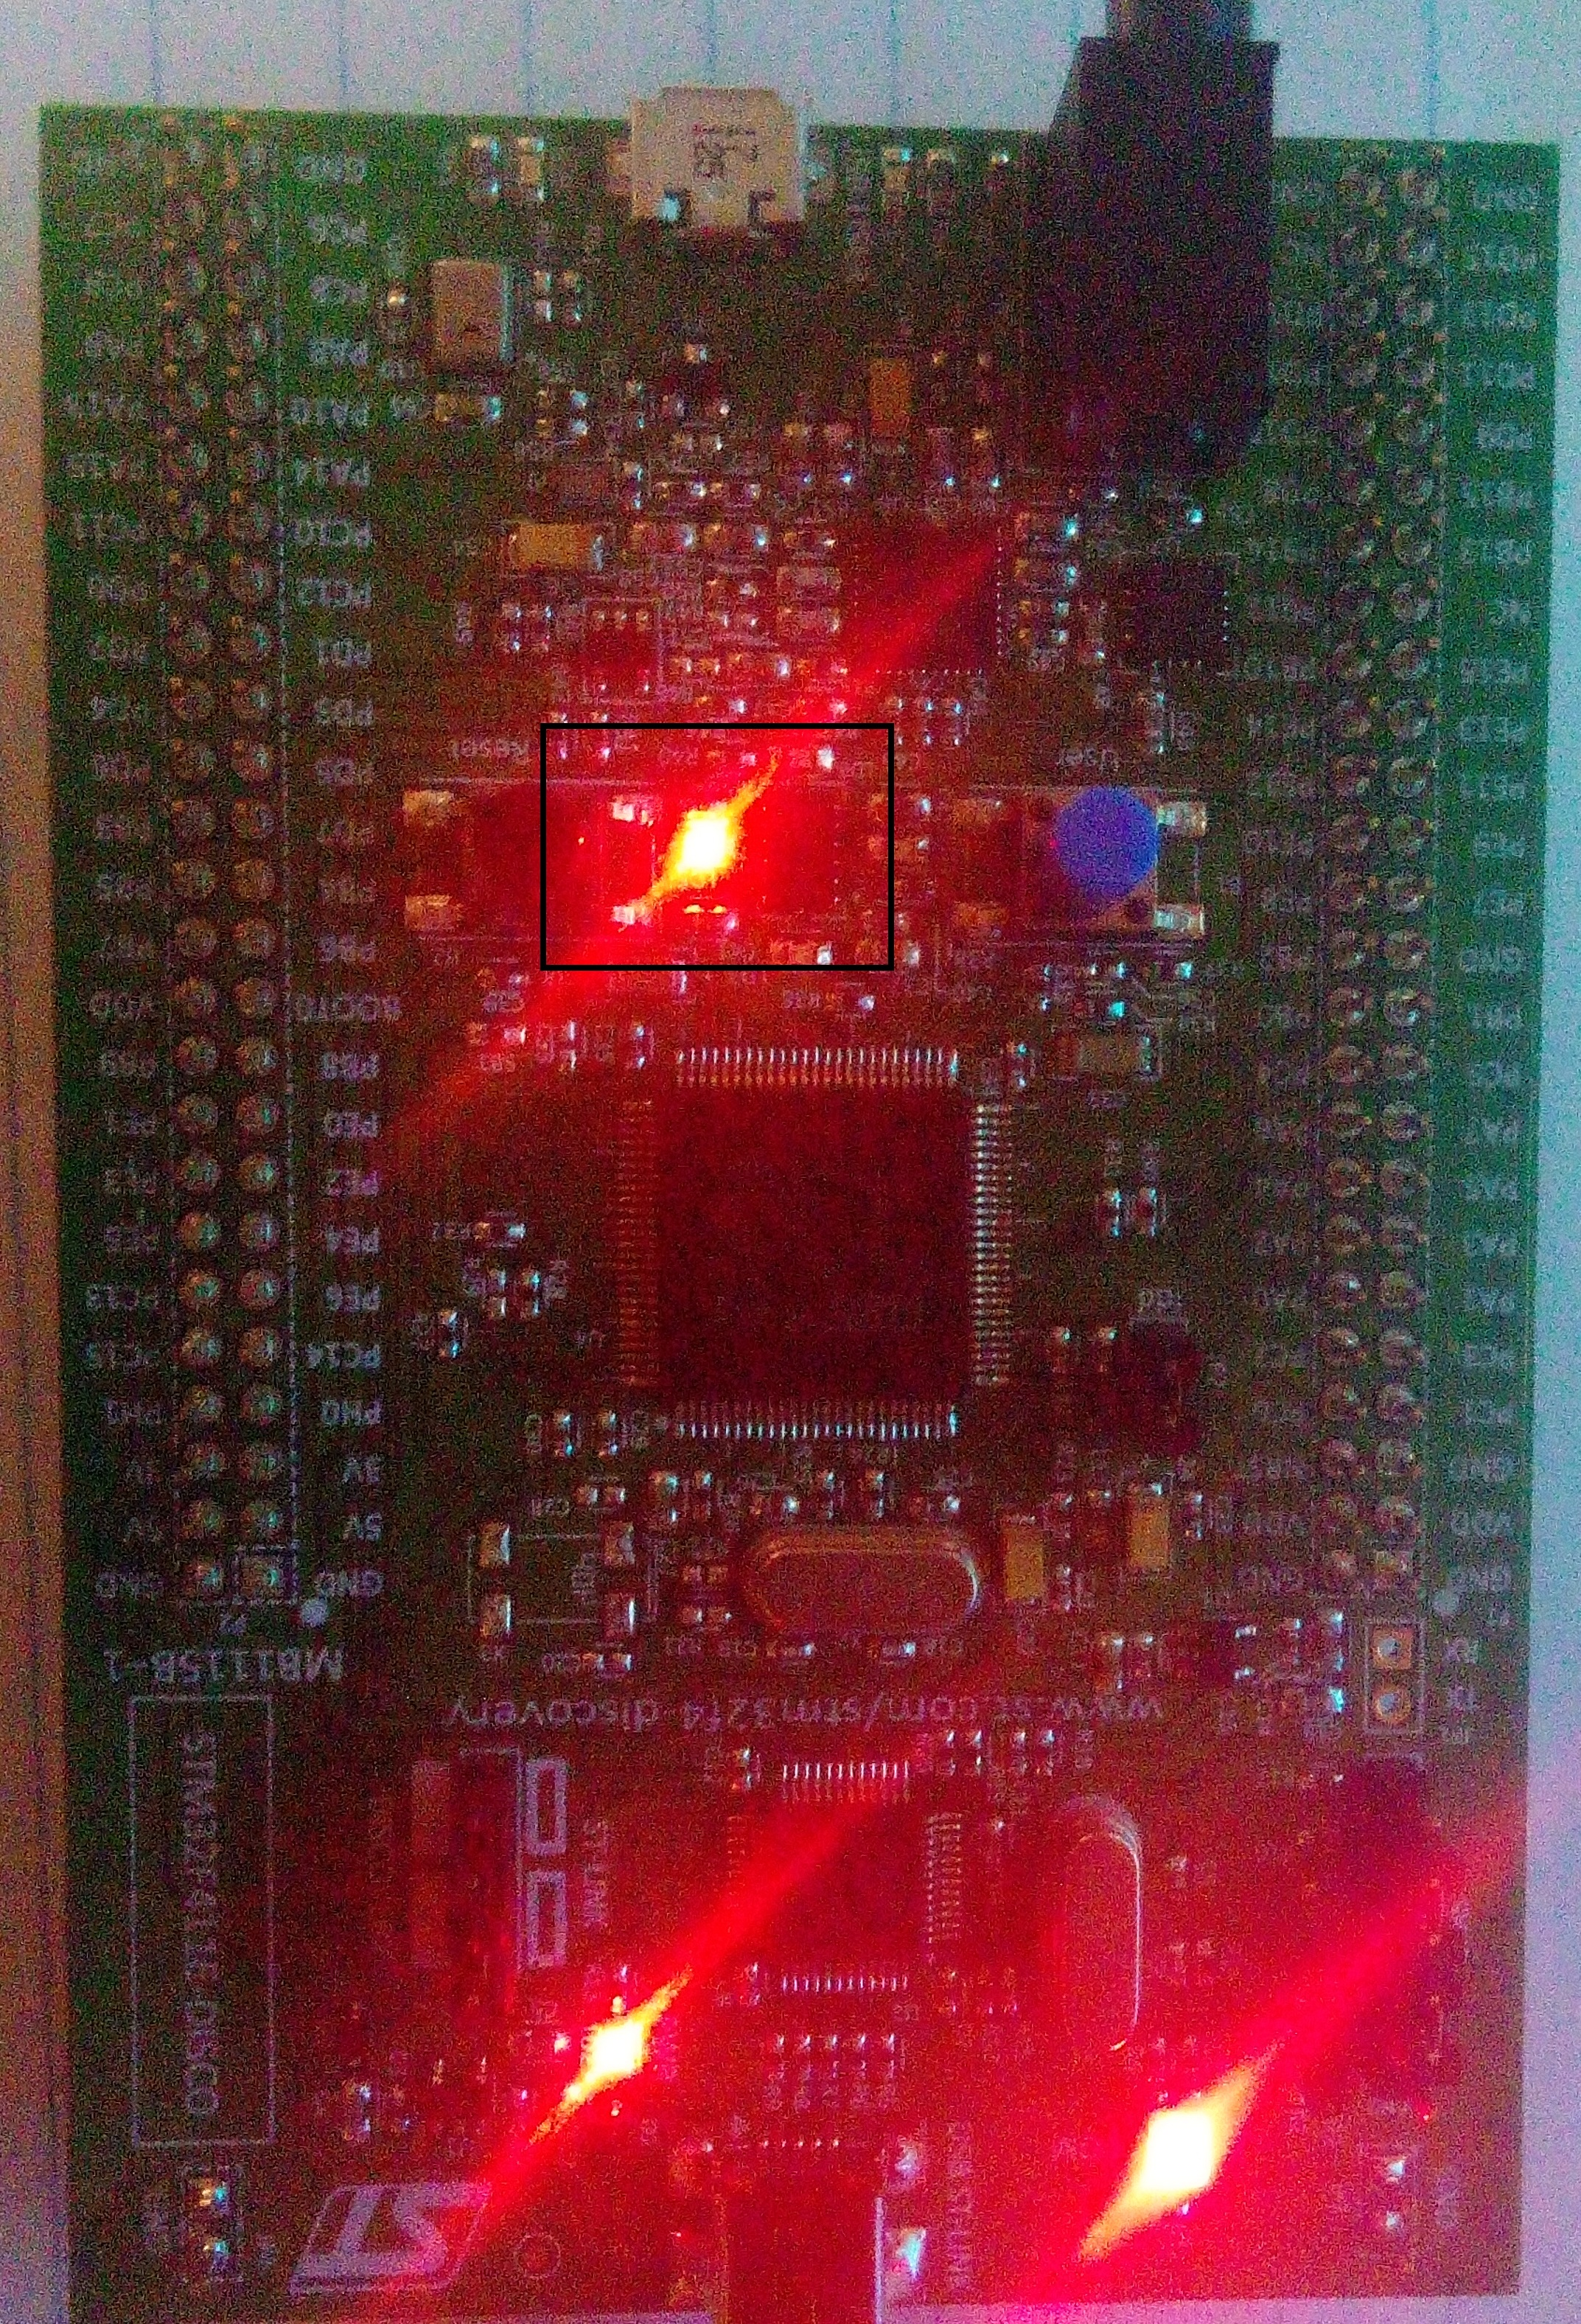
\includegraphics[width = 30mm, angle = 90]{re3.jpg}
\caption{Flashing red LED on real world MCU}
\label{re3.1}
\end{center}
\end{figure}

Figure~\ref{re3.1}, shows the blinking LED functionality on a real world MCU, namely the SMT32F411E. If this behaviour can be mimicked in the emulator, a promising solution to the problem in \textbf{\ref{ps} \nameref{ps}}, will have been found. Figure~\ref{re3.2} illustrates the code required for the blinking of the red LED in STM32CubeIDE.

\begin{figure}[H]
\begin{center}
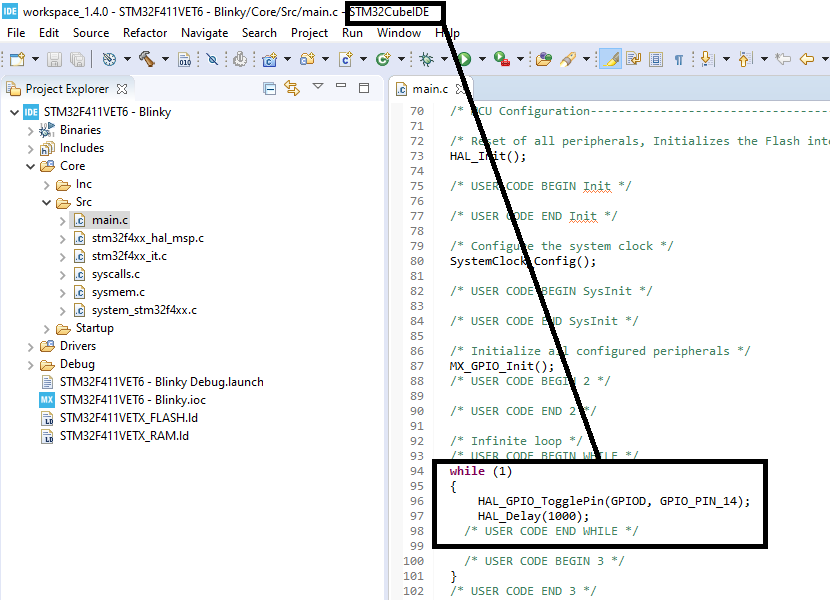
\includegraphics[width = 100mm]{re3.png}
\caption{Code in STM32CubeIDE to introduce LED blinking}
\label{re3.2}
\end{center}
\end{figure}




\subsection{Emulated MCU in Eclipse Embedded CDT}
\label{real}

\begin{figure}[H]
\begin{center}
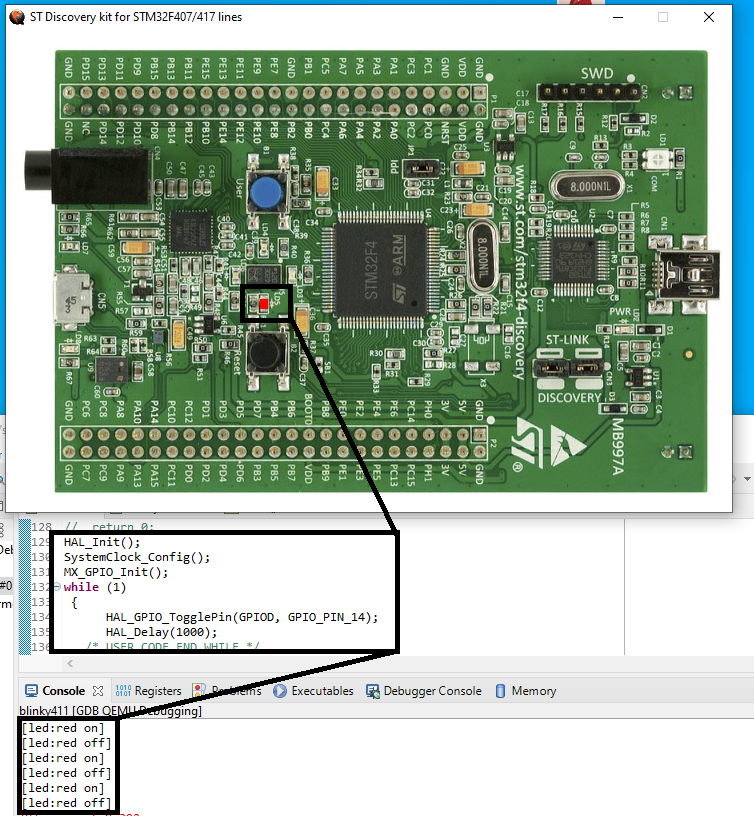
\includegraphics[width = 90mm]{re2.png}
\caption{Flashing red LED in emulated environment using code from STM32CubeIDE}
\label{re2}
\end{center}
\end{figure}

Figure~\ref{re2}, shows that the emulation process (using the same code as produced in STM32CubeIDE) is successful. The depicted basic functionality works on the emulator, despite it being a different MCU than the one used in STM32CubeIDE.

\section{Autonomous code evaluation results} 
\label{codRes}

The three step autonomous system was described extensively in \textbf{\nameref{4detailedd}}. In this section the results of the system will be illustrated.

\subsection{Step1 results}
\label{1res}

\begin{figure}[H]
\begin{center}
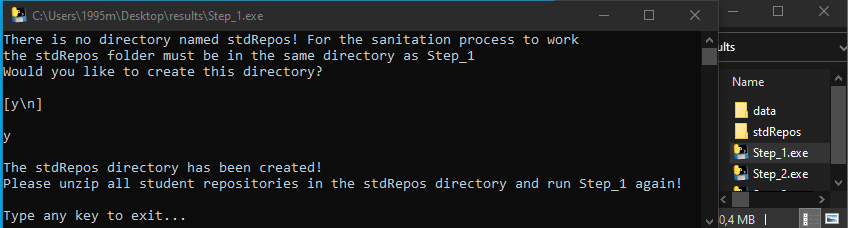
\includegraphics[width = 155mm]{r1.png}
\caption{Results after the first iteration of Step1}
\label{r1}
\end{center}
\end{figure}

Observable from Figure~\ref{r1}, is the state of the root directory (where the .py/.exe files are stored) after the first iteration of Step1.py/.exe. It can be seen that a terminal prompt appears requesting the user to create the "stdRepos" directory. Furthermore, the "data" directory is created within the program root directory. The user is instructed to unzip directories in the "stdRepos" folder.

\begin{figure}[H]
\begin{center}
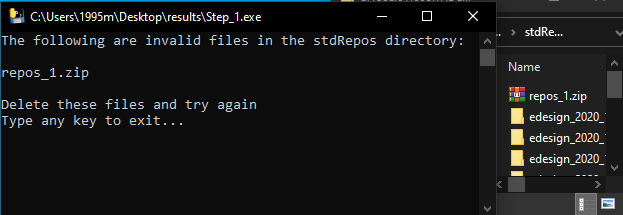
\includegraphics[width = 155mm]{r2.png}
\caption{Results after the second iteration of Step1}
\label{r2}
\end{center}
\end{figure}

Figure~\ref{r2}, displays the programs ability to detect unwanted files in the "stdRepos" directory. It can be observed that the required repositories have been unzipped, but the zipped file has not yet been deleted. The terminal prompts the user to do so and rerun Step1.py/.exe.

\begin{figure}[H]
\begin{center}
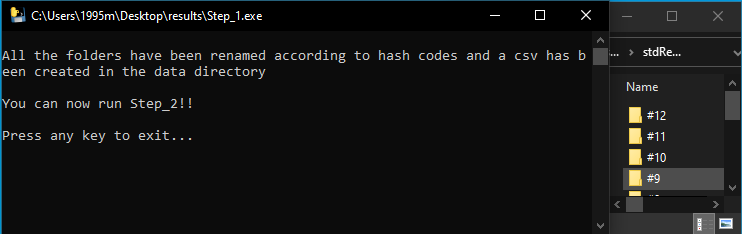
\includegraphics[width = 155mm]{r3.png}
\caption{Results after the third iteration of Step1}
\label{r3}
\end{center}
\end{figure}

Finally Figure~\ref{r3}, illustrates the renaming of the folder within the "stdRepos" directory in order to uphold anonymity as discussed previously. Furthermore, it can be seen that the terminal once again guides the user to the next step in the autonomous system.

\subsection{Step2 results}
\label{2res}

\begin{figure}[H]
\begin{center}
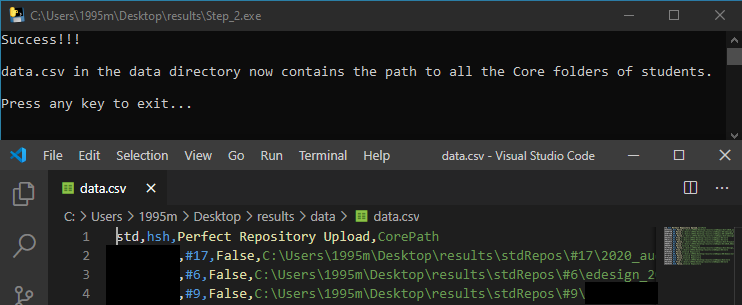
\includegraphics[width = 110mm]{r4.png}
\caption{Results after Step2}
\label{r4}
\end{center}
\end{figure}

Figure~\ref{r4} illustrates the state of the data.csv file within the "data" directory after the successful execution of Step2.py/.exe. It can be seen that the absolute path to the core folder is stored according to unique student identifiers. Student numbers in Figure~\ref{r4} have been censored for the sake of anonymity.

\subsection{Step3 results}
\label{3res}

\begin{figure}[H]
\begin{center}
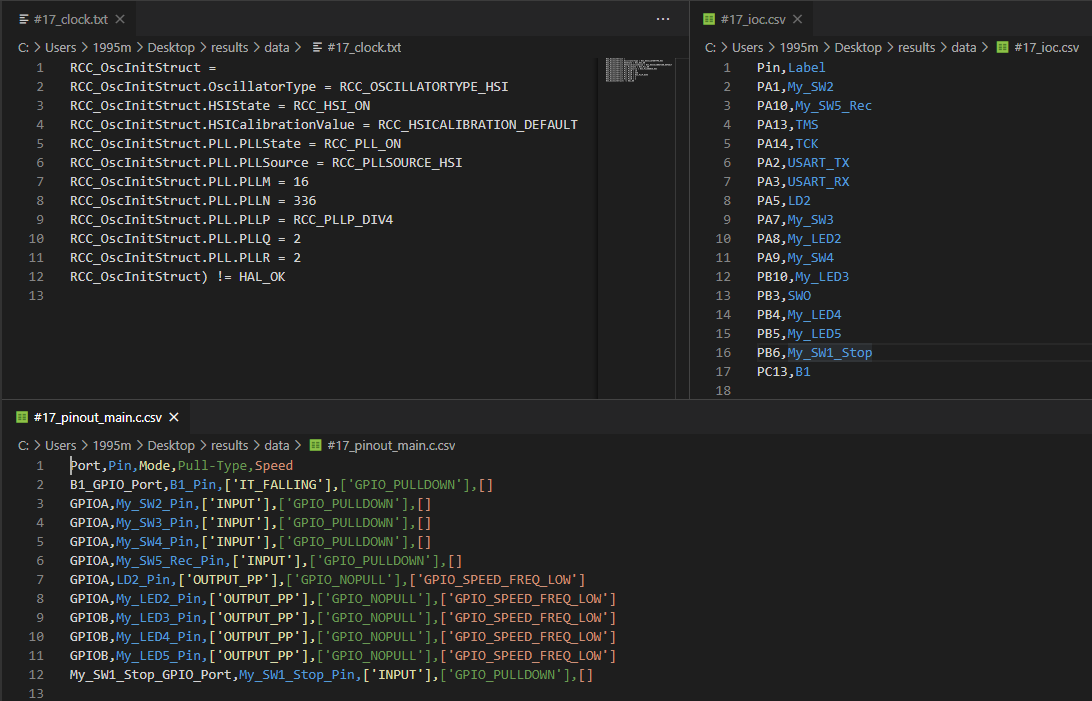
\includegraphics[width = 155mm]{r5.png}
\caption{Results after Step3}
\label{r5}
\end{center}
\end{figure}

The final step of the autonomous system produces the results depicted in Figure~\ref{r5}. The content of the three files outlined in \textbf{\ref{step3} \nameref{step3}}, are displayed for a specific student. It can be seen that the entire clock configuration is extracted and saved in addition to the pin configurations. It is, furthermore, observable that students often label pins within STM32CubeIDE. This makes it difficult to evaluate code, since pin numbers are not displayed in main.c when custom labels are applied. By extracting pin information from the .ioc files, however, the custom labels can be associated with specific pin numbers are seen in Figure~\ref{r5}.\newpage\cleardoublepage


\chapter*{6 Conclusion}
\label{6conc}
\addcontentsline{toc}{chapter}{6 Conclusion}
\setcounter{chapter}{6}
\setcounter{section}{0}
\setcounter{figure}{0}
\setcounter{table}{0}

This chapter highlights and reiterates the achieved objectives, results and future recommendations of the project. It should be read in conjunction with \textbf{\nameref{intro}} and is reconcilable with the mentioned chapter.

\section{Objectives achieved}
The problem statement as illustrated in \textbf{\ref{ps} \nameref{ps}}, is achieved by fulfilling the objectives of this project. If these objectives are indeed adequately fulfilled, the problem stated will have been resolved.

\subsection{Emulator/simulator investigation}
It was illustrated in \textbf{\nameref{2emul}} and \textbf{\ref{emuRes} \nameref{emuRes}}, that it is indeed possible, with enough effort, to mimic real-world MCU behaviour on a chosen emulator. The implications of this are readily apparent.
\\\\
If simple functionality (such as a blinking LED) can be replicated within the QEMU emulator as detailed in \textbf{\nameref{2emul}}, any functionality could theoretically be replicated to some degree of accuracy. 
\\\\
It was clearly illustrated in \textbf{\nameref{2emul}} that the blinking LED functionality can be replicated in an emulated environment. The objective as stated in \textbf{\ref{emInvestObj} \nameref{emInvestObj}} has thus been achieved.

\subsection{Autonomous high-level code structure evaluation}
\textbf{\ref{highLevObj} \nameref{highLevObj}} states a second objective of this project. Once this second objective has been achieved, the problem as stated in \textbf{\ref{ps} \nameref{ps}} has been fully resolved.
\\\\
The subject of \textbf{\nameref{system3}} and \textbf{\nameref{4detailedd}}, is the achievement of this objective. It is quite apparent from the previously mentioned chapters, in conjunction with \textbf{\ref{codRes} \nameref{codRes}}, that this objective has been achieved. 
\\\\
Varying student code can easily be evaluated in terms of MCU configurations in an autonomous way. It is important to note that pin and clock configurations were chosen to illustrate this achieved aim. It is however possible to extend this functionality to any high level code structures by simply tweaking the python code (specifically the regular expressions discussed) to search for different patterns.
\\\\
The second objective of this project has thus been met. The problem statement has been resolved and a novel solution has been applied to a dynamic problem.

\section{Recommendations}

As described in \textbf{\ref{scOfWrk} \nameref{scOfWrk}}, and as a result of the limited time available for this project, certain constraints had to be introduced. For future work, in addressing the topic at hand, it is recommended that some of these limitations are lifted. 
\\\\
Firstly, it is of note that the list of supported MCUs for various emulators will change over time. It is, therefore, recommended that future projects in a similar vain to this one, re-assess the list of supported MCUs for the various emulators. Of particular interest is the planned future support of the STM32 Nucleo range by the xPack Arm QEMU Project. In conjunction with the aforementioned, it is recommended that the other emulators mentioned in this project, be further investigated as time passes and development continues.
\\\\
In addition, the chosen functionality to recreate in the emulator involved a flashing LED. It was indeed outside the scope of this project to recreate more advanced functionalities within the described frameworks of \textbf{\nameref{2emul}}. More functionality can thus be introduced by future endeavours (given that solutions supporting more peripherals are discovered).
\\\\
It can be seen from \textbf{\ref{codRes} \nameref{codRes}}, that a simple terminal is used to guide the user in the process of autonomous code evaluation. This was done to facilitate the process of automation, but required some manual interaction by the user. It is hence recommended, for the sake of automation, that future projects reduce the extent of these manual interactions. This can be done using a GUI or an autonomous execution chain.
\\\\
Furthermore, the evaluation of student code is limited in this project. Evaluation occurred for pin and clock configurations exclusively due to time and scope constraints. It is recommended that succeeding investigations extend the scope of the evaluation to include further configurations (like UART). 
\\\\
Lastly, this project addressed the problem statement in a two-part, mutually exclusive way. The investigation of the emulator was not dependant on, nor relevant to, the evaluated code. A future project might, therefore, consider recreating student MCU functionality on a chosen emulator in its totality. Implementing the aforementioned functionality is, indeed, a very extensive task and should perhaps be the topic of an entire project.


\newpage\cleardoublepage
\chapter*{}
\label{bib}
\addcontentsline{toc}{chapter}{References}

\bibliography{bib/thesis.bib}
\bibliographystyle{ieeetr}
\chapter*{Appendix A: Project planning schedule}
\label{A}
\addcontentsline{toc}{chapter}{Appendix A: Project planning schedule}


\chapter*{Appendix B: Outcomes compliance}
\label{B}
\addcontentsline{toc}{chapter}{Appendix B: Outcomes compliance}
\chapter*{Appendix C}
\label{C}
\addcontentsline{toc}{chapter}{Appendix C}
\chapter*{Appendix D}
\label{D}
\addcontentsline{toc}{chapter}{Appendix D}
\end{document}

